\problemname{Pyramidebyggeri}

\begin{figure}[h!]
  \centering
  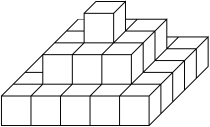
\includegraphics[scale=1.5]{pyramid}
\end{figure}

Inden man går i gang med et større projekt, fx at bygge en pyramide, er det en god idé at tænke sig om en ekstra gang.
Du skal skrive et program der udregner, hvor høj en pyramide du kan bygge med et vist antal stenblokke.

Vi antager, at pyramiden er kompakt, dvs.\ at der ikke findes hulrum indeni.
Desuden er den konstrueret som vist i ovenstående figur.
Hvert lag er altså kvadratisk, og dets sidelængde er to blokke mindre end det underliggende lags.
Det øverste lag består altid af en enkelt stenblok.

Programmet skal indlæse antallet af tilgængelige stenblokke (højst hundrede millioner) og udskrive højden (målt i antal stenblokke) for den højeste pyramide som kan bygges.
Det gør ikke noget, at der bliver blokke tilovers, men der må ikke mangle en eneste blok.

\section*{Indlæsning}
Indlæsningen er et enkelt heltal: antallet af forhåndenværende stenblokke.

\section*{Udskrift}
Programmet skal skrive en linje med et enkelt heltal: højden af den højeste pyramide som kan bygges med de forhåndenværende stenblokke.
